\documentclass[aspectratio=169]{beamer}
\beamertemplatenavigationsymbolsempty

\usepackage{parskip, setspace}
\setstretch{1.25}

\usepackage{biblatex}
\addbibresource{bib.bib}
% math formatting
\usepackage{amsmath, amsfonts, braket}
% \numberwithin{equation}{section}
% rich text
\usepackage{graphicx, caption}
\usepackage{hyperref}
\usepackage{xcolor}
\hypersetup{
    colorlinks=true,
    linkcolor=black,  
    urlcolor=blue,
    citecolor=blue,
    pdftitle={A Survey of Computational Physics},
    pdfpagemode=FullScreen
}

\usepackage[ruled,linesnumbered,lined,boxed,commentsnumbered]{algorithm2e}

\usetheme{Madrid}
\title[Quantum Computing]{Quantum Computing}
% \subtitle{}

\author[Chapman, Nathan]{Nathan Chapman}

\institute[CWU]
{
%   Faculty of Physics\\
  Central Washington University
%   \and
%   \inst{2}%
%   Faculty of Chemistry\\
%   Very Famous University
}

\date[HPC 2024]{CS 530: High Performance Computing, Spring 2024}

\logo{
\includegraphics[height=0.5cm]{images/cwu_logo.png}}

\begin{document}

\frame{\titlepage}

\begin{frame}
    \frametitle{Why do we care?}
    \begin{columns}
        \begin{column}{0.5\textwidth}
            \begin{itemize}
                \item Because it's cool
                \item It turns out quantum computers can easily break classical cryptography
            \end{itemize}
        \end{column}
        \begin{column}{0.5\textwidth}
            
        \end{column}
    \end{columns}
\end{frame}

\begin{frame}
    \frametitle{Qubits - Heads or Tails?}

    \centering
    Does a coin show heads or tails?

\end{frame}

\begin{frame}
    \frametitle{Qubits - Single}
    \begin{columns}
        \begin{column}{0.5\textwidth}
            \begin{itemize}
                \item Classical - ``Bit''
                    \begin{itemize}
                        \item State is true or false
                        \item Always
                    \end{itemize}
                \item Quantum - ``Qubit''
                    \begin{itemize}
                        \item State is true or false or tralse or frue
                        \item State is a little bit of both
                        \item Until measured
                        \item At measurement, the state is true or false
                        % \item Example
                        % \begin{itemize}
                        %     \item Quantum Coin
                        %     \item $\ket{+} = \frac{1}{\sqrt{2}} \ket{0} + \frac{1}{\sqrt{2}} \ket{1}$
                        %     \item 50-50 probability
                        % \end{itemize}
                    \end{itemize}
                \item Example - A simple coin
                    \begin{itemize}
                        \item Classical - Deterministic via applied force, torque, height, etc.
                        \item Quantum - Probabilistic until measured
                    \end{itemize}
            \end{itemize}
        \end{column}
        \begin{column}{0.5\textwidth}
            \begin{figure}[h]
                \centering
                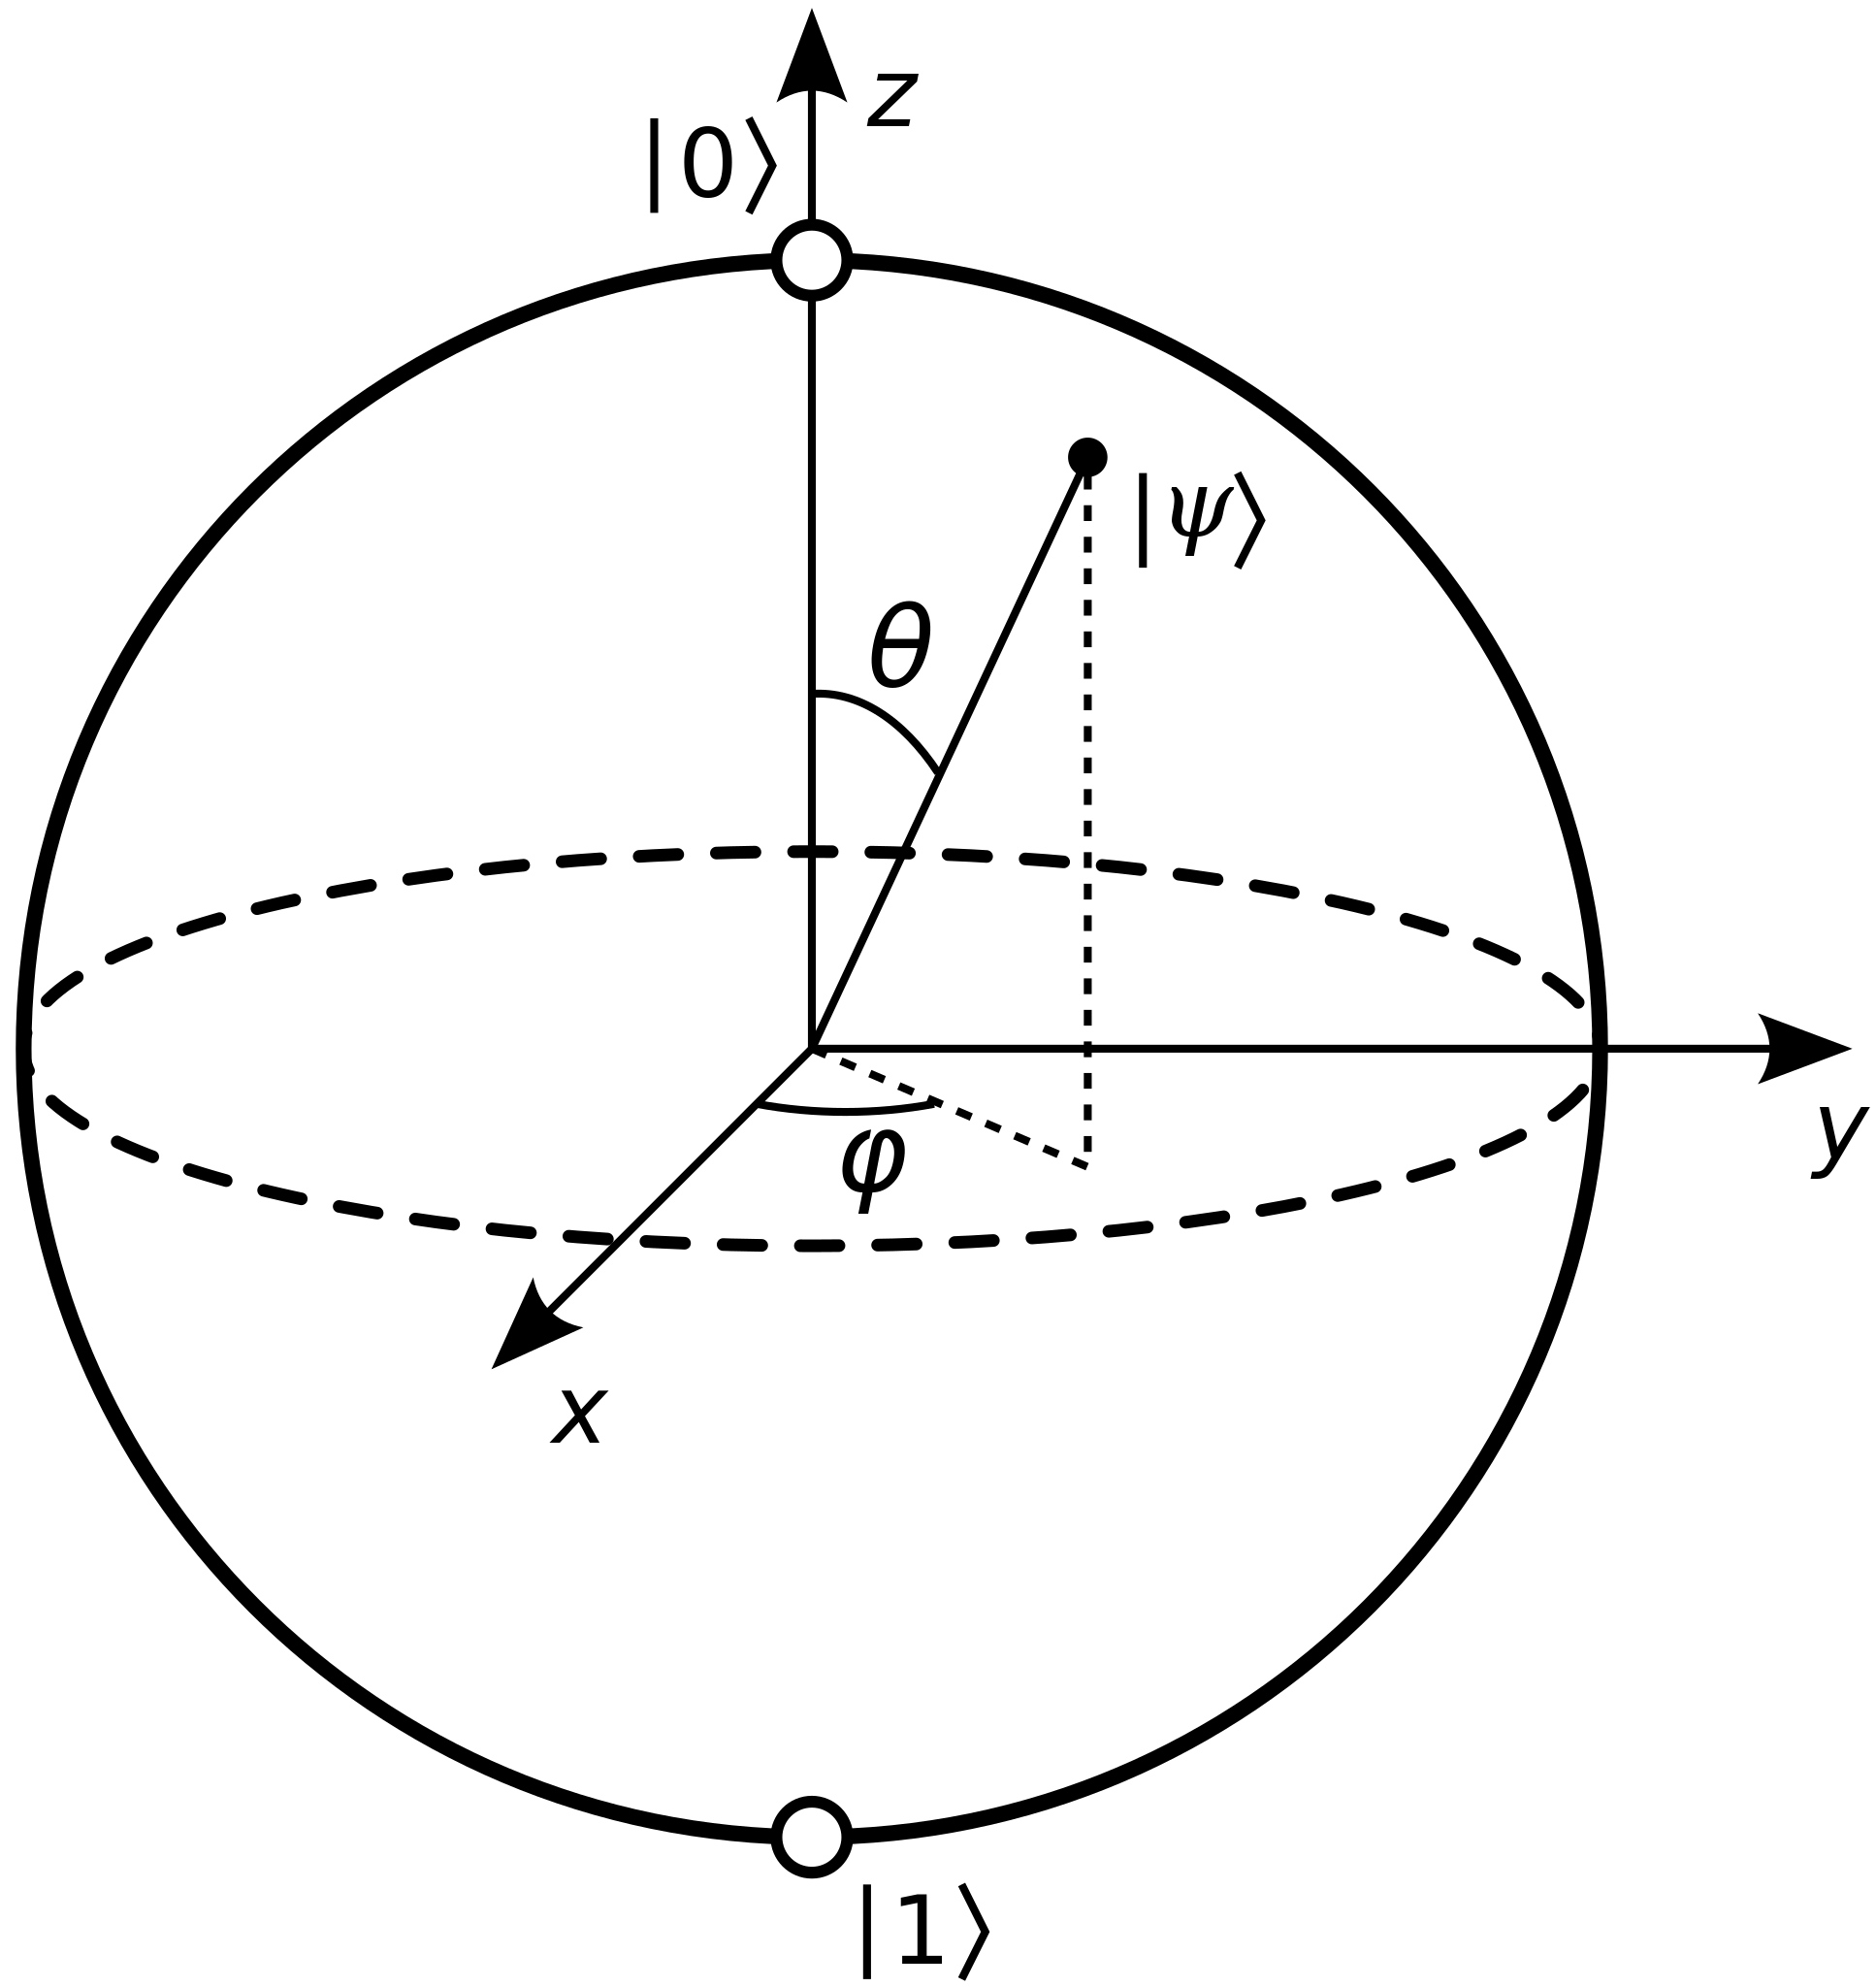
\includegraphics[height=0.7\textheight]{images/Bloch_sphere.png}
                \caption{The Bloch sphere reprensetation of a qubit \\ $\ket{\psi} = \cos \left( \frac{\theta}{2} \right) \ket{0} + e^{i \phi} \sin \left( \frac{\theta}{2} \right) \ket{1}$}
            \end{figure}
        \end{column}
    \end{columns}
\end{frame}

\begin{frame}
    \frametitle{Qubits - Multiple}
    \begin{columns}
        \begin{column}{0.5\textwidth}
            \begin{itemize}
                \item 2 qubits $\implies$ state is a mix between the 4 permutations $\{\ket{00}, \ket{01}, \ket{10}, \ket{11} \}$
                \item Each permutation has its own probability such that the total is 1
                \item Measure only qubit $\implies$ state renormalizes to only include remaining possible states
                \item Bell State: $50\% \ket{00}$ and $50\% \ket{11}$
            \end{itemize}
        \end{column}
        \begin{column}{0.5\textwidth}
            \centering Demo: 2 quantum coins with a volunteer
        \end{column}
    \end{columns}
\end{frame}

\begin{frame}
    \frametitle{Qubits - Quantum Registers}
    \begin{columns}
        \begin{column}{0.5\textwidth}
            \centering{\underline{Classical}}
            \begin{itemize}
                \item Register of size $N \equiv N$ flip-flops
                \item Stores 1 permutation of states
            \end{itemize}
        \end{column}
        \begin{column}{0.5\textwidth}
            \centering{\underline{Quantum}}
            \begin{itemize}
                \item Register of size $N$ $\equiv$ $N$ qubits
                \item Stores ALL $2^N$ permutations of states
            \end{itemize}
        \end{column}
    \end{columns}
    \begin{block}{}
        \centering The information density of a quantum computer can be massive
    \end{block}
\end{frame}

\begin{frame}
    \frametitle{Quantum Computation - Single Qubit Gates}
    \begin{columns}
        \begin{column}{0.5\textwidth}
            \centering{\underline{Classical}}
            \begin{itemize}
                \item Only one non-trivial gate
                \item NOT - $0 \to 1$
            \end{itemize}
        \end{column}
        \begin{column}{0.5\textwidth}
            \centering{\underline{Quantum}}
            \begin{itemize}
                \item Several non-trivial gates
                \item NOT (X) - swaps the probabilities
                \item Z - flips the sign of the probability on the $\ket{1}$ state
                \item Hadamard - ``mixes'' the pure states toward the other
                    \begin{itemize}
                        \item $\ket{0} \to 50\% \ket{0}$ and $50\% \ket{1}$
                        \item $\ket{1} \to 50\% \ket{0}$ and $-50\% \ket{1}$
                    \end{itemize}
            \end{itemize}
        \end{column}
    \end{columns}
\end{frame}

\begin{frame}
    \frametitle{Quantum Computation - Single Bit Gates}
    \begin{figure}[h]
        \centering
        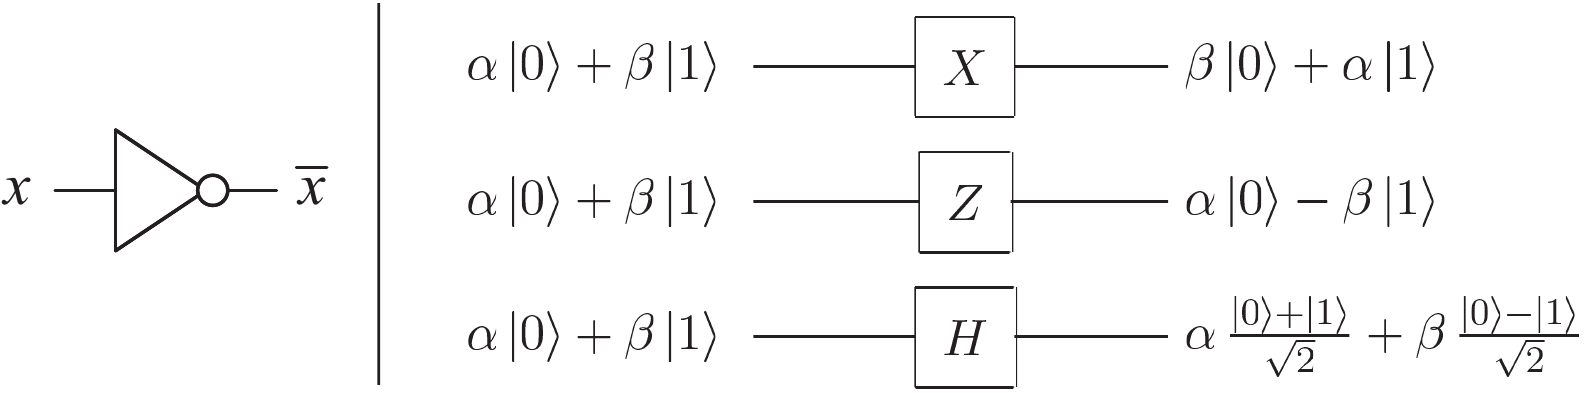
\includegraphics[width=0.9\textwidth]{images/single_circuits.png}
        \caption{A comparison between logic gates that can act on a single classical or quantum bit.}
    \end{figure}
\end{frame}

\begin{frame}
    \frametitle{Quantum Computation - Multi-Qubit Gates}
    \begin{columns}
        \begin{column}{0.5\textwidth}
            \centering{\underline{Classical}}
            \begin{itemize}
                \item AND, OR, XOR, NAND, NOR
                \item[]
                \item[]
                \item[] 
                \item XOR isn't invertible
                \item NAND makes up all gates
            \end{itemize}
        \end{column}
        \begin{column}{0.5\textwidth}
            \centering{\underline{Quantum}}
            \begin{itemize}
                \item Controlled not - CNOT
                \item Uses a \emph{control} bit and a \emph{target}
                \item If control is 1, NOT target, otherwise do nothing
                \item CNOT is invertible
                \item CNOT and single-gates make up all multi-gates
            \end{itemize}
        \end{column}
    \end{columns}
    \begin{alertblock}{}
        \centering Quantum gates need to conserve information
    \end{alertblock}
\end{frame}

\begin{frame}
    \frametitle{Quantum Computation - Circuits}
    \begin{columns}
        \begin{column}{0.5\textwidth}
            \begin{itemize}
                \item Sequence of gates
                \item Read left to right
                \item Lines are ``wires''
                \item No loops
                \item Wires can't connect to conserve information
                \item Can connect from one bit (black dot) to a target bit ($\oplus$)
                \item $\oplus$ represents addition mod 2 
            \end{itemize}
        \end{column}
        \begin{column}{0.5\textwidth}
            \begin{figure}[h]
                \centering
                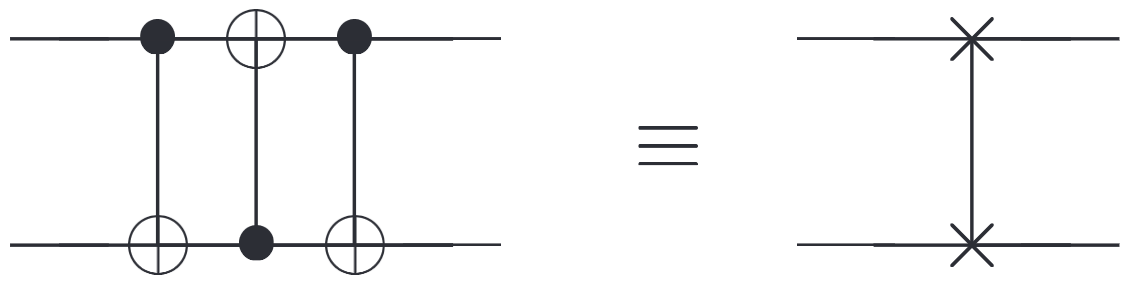
\includegraphics[width=\textwidth]{images/swap_circuit.png}
                \caption{A quantum circuit to swap the states of two given qubits (left) and its compact notation (right).}
            \end{figure}
        \end{column}
    \end{columns}
\end{frame}

\begin{frame}
    \frametitle{Quantum Algorithms - The Quantum Fourier Transform}
    \begin{columns}
        \begin{column}{0.5\textwidth}
            \begin{itemize}
                \item Classical DFT $y_k \equiv \dfrac{1}{\sqrt{N}} \sum\limits_{j = 0}^{N - 1} e^{2 \pi i j k / N} x_j$
                \item FFT uses $\Theta(N 2^N)$ gates
                \item Quantum FT $\ket{j} \to \dfrac{1}{\sqrt{2^N}} \sum\limits_{k = 0}^{2^N - 1} e^{2 \pi i j k / 2^N} \ket{k}$
                \item QFT uses $\Theta(N^2)$ gates
            \end{itemize}
        \end{column}
        \begin{column}{0.5\textwidth}
            \begin{figure}
                \centering
                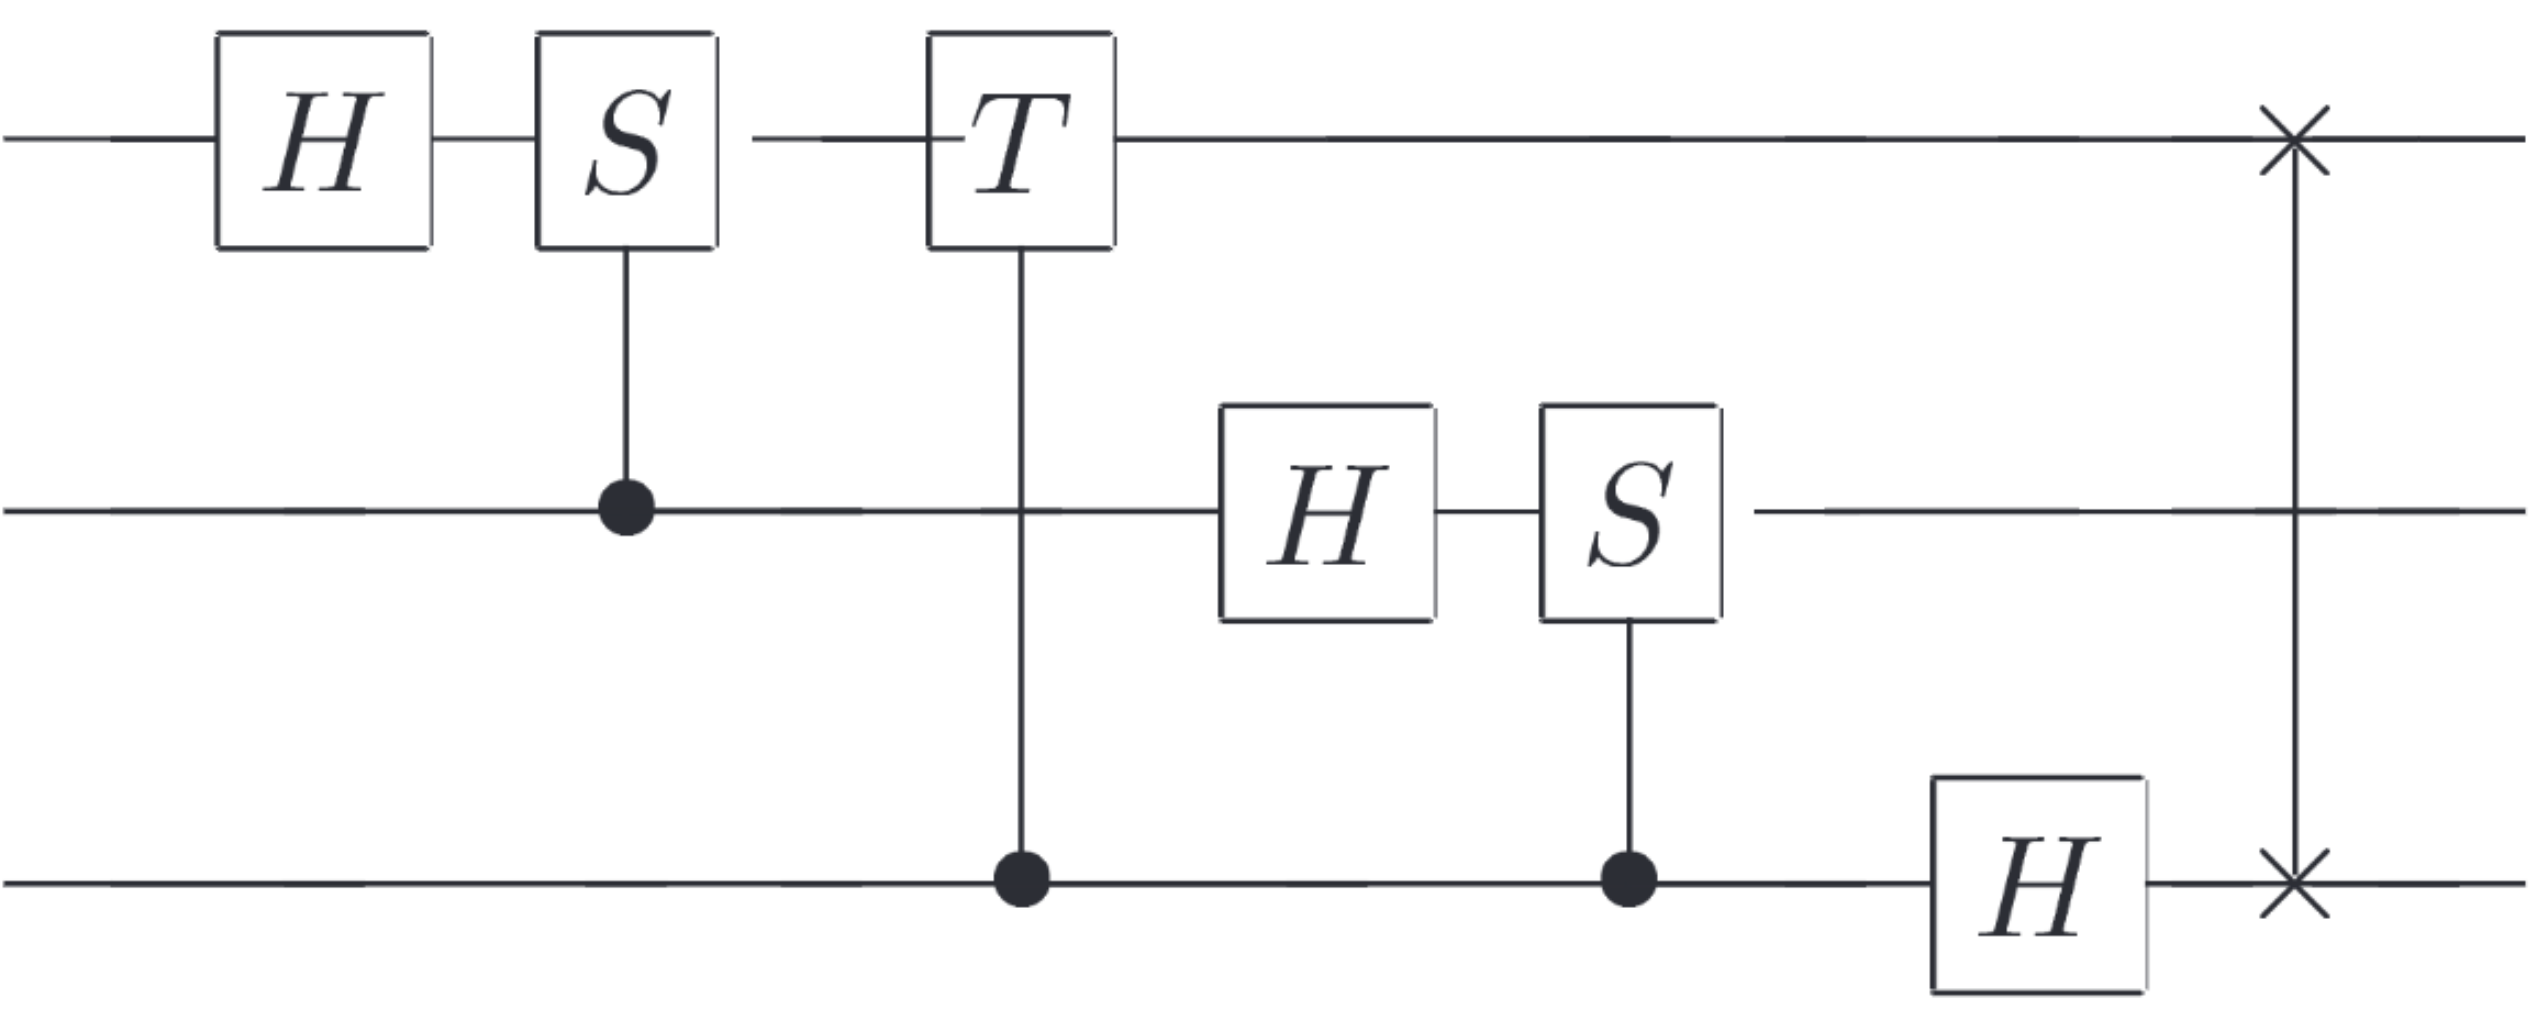
\includegraphics[width=\textwidth]{images/QFT_3bit.png}
                \caption{A 3-qubit quantum Fourier transform circuit.  $S,T$ are the phase and $\pi/8$ gates, respectively.}
            \end{figure}
        \end{column}
    \end{columns}
    \begin{alertblock}{}
        \centering Quantum computers calculate the Fourier Transform with \emph{exponentially} fewer operations
    \end{alertblock}
\end{frame}

% \begin{frame}
%     \frametitle{Quantum Cryptography}
%     \begin{columns}
%         \begin{column}{0.5\textwidth}
            
%         \end{column}
%         \begin{column}{0.5\textwidth}
            
%         \end{column}
%     \end{columns}
% \end{frame}

\begin{frame}
    \frametitle{Demo - Qiskit}
    \begin{columns}
        \begin{column}{0.5\textwidth}
            \begin{itemize}
                \item Many quantum cloud computing platforms
                \item Most popular is Qiskit by IBM
                \item Allows jobs to be submitted to IBM's quantum computer with ~127 qubits
                \item Demo
            \end{itemize}
        \end{column}
        \begin{column}{0.5\textwidth}
            \begin{figure}[placement]
                \centering
                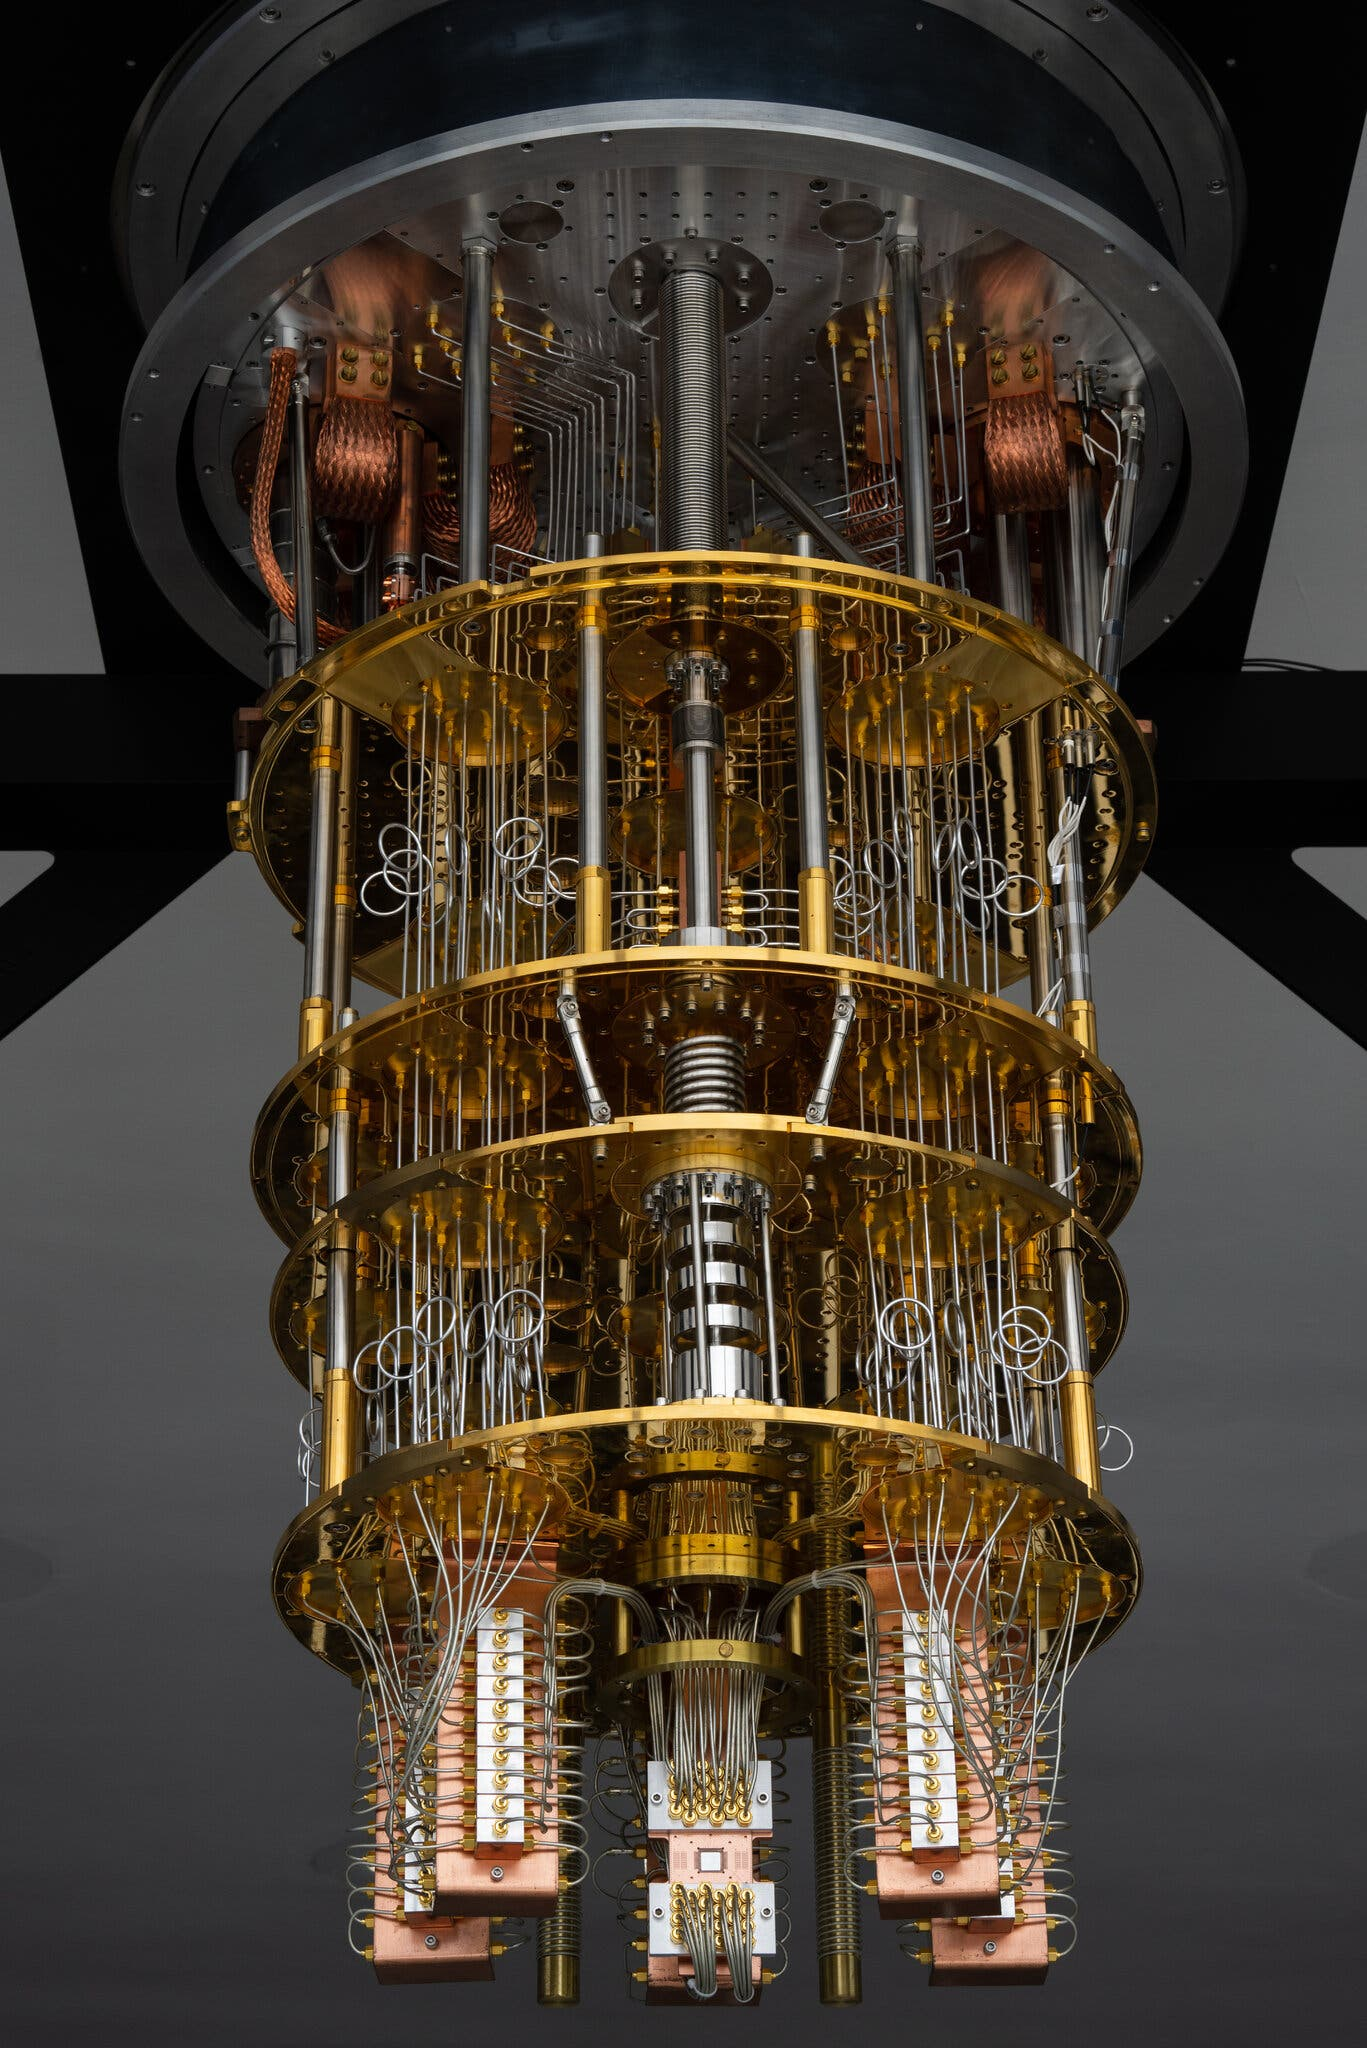
\includegraphics[height=0.66\textheight]{images/quantum_computer.jpg}
                \caption{A real quantum computer} %\href{https://www.nytimes.com/2023/06/14/science/ibm-quantum-computing.html}{SOURCE}}
            \end{figure}
        \end{column}
    \end{columns}
\end{frame}

\begin{frame}
    \frametitle{Conclusion}

    \begin{itemize}
        \item Quantum computation is different at the most fundamental levels
        \item A collection of $N$ qubits stores $2^N$ values
        \item Every quantum gate can be made of CNOT and single-qubit gates
        \item Quantum gates conserve information
        \item A quantum circuit is a sequence of applied quantum gates
        \item The quantum Fourier Transform requires exponentially fewer operations
        \item There are real quantum computers in the world and we can use them with Qiskit!
    \end{itemize}

\end{frame}

\end{document}